\subsection{Context Closure}
\label{sec:context_closure}
% It is crucial to ensure that the weight of any object subject to rewriting is greater than or equal to $1_\mathcal{S}$.
% This issue is addressed by the existence of a context closure. Specifically, it ensures that every graph that can be rewritten using that rule admits some morphism into the weighted type graph, and thus the weight of the morphism, which is the sum of the weights of the morphisms into the type graph, is greater than or equal to \(1_S\) by the following~\autoref{lem:wf:morphism_weight_geq_1_neq_0}.

It is crucial to ensure that the weight of any object subject to rewriting is not $0_S$, because \(0_S\) behaves unpredictably in strongly monotonic measurable semirings. For instance, in the natural tropical semiring \((\mathbb{N} \mathop{\cup} \{\mathop{+\infty}\}, \mathop{\min}, +)\), the element \(0_S\) is the greatest element \(\mathop{+\infty}\), while in the natural arctic semirings \((\mathbb{N} \mathop{\cup} \{\mathop{-\infty}\}, \max, +)\), the element \(0_S\) is the smallest element \(\mathop{-\infty}\).
This issue is addressed by the existence of a context closure defined as follows:

% \begin{lemma}[Lemma 4.5~\cite{endrullis2024generalized_arxiv_v4}]
% \label{lem:wf:morphism_weight_geq_1_neq_0}
% Let $\mathcal{T} \mathop{=} (T, \mathbb{E}, S, \mathbf{w})$ be a finitary weighted type graph. Then
% \begin{itemize}
%     \item for every $\phi : G \mathop{\to} T$: $1_S \mathop{\preceq} \mathbf{w}_\mathcal{T}(\phi) \mathop{\neq} 0_S$;
%     \item for every $\phi : G \mathop{\to} T$ and $\alpha : A \mathop{\to} G$: $1_S \mathop{\preceq} \mathbf{w}_\mathcal{T}(\phi - (\alpha \circ -)) \mathop{\neq} 0_S$;
% \end{itemize}
% \end{lemma}
% \begin{remark} 
%   \label{remark:semiring_0_unpredictable}
%   The requirement \textquote{for all \(e \mathop{\in} \mathbb{E}, w(e) \mathop{\neq} 0_S\)} is necessary because \(0_S\) behaves unpredictably in strongly monotonic measurable semirings. For instance, in the natural and real tropical semirings \((\mathbb{N} \mathop{\cup} \{\mathop{+\infty}\}, \mathop{\min}, +)\), \(0_S\) is the greatest element \(\mathop{+\infty}\), while in the natural and real arctic semirings \((\mathbb{N} \mathop{\cup} \{\mathop{-\infty}\}, \max, +)\), \(0_S\) is the smallest element \(\mathop{-\infty}\).
% \end{remark} 

\begin{definition}[\cite{endrullis2024generalized_arxiv_v2}]
    \label{def:context_closure}  
    Let $\mathcal{T}=(T,\mathbb{E},\mathcal{S},w)$ be a finitary weighted type graph, \(\rho \mathop{=} (L \overset{l}{\leftarrow} K \overset{r}{\rightarrow} R ) \) a DPO rewriting rule and $\mathfrak{F}$ a rewriting framework. 
    A \textbf{context closure} for $\rho$ and $\mathcal{T}$ in $\mathfrak{F}$ is a morphism $c:L \mathop{\rightarrow} T$ such that for every DPO diagram in $\mathfrak{F}(\rho)$ shown below,
    there is $\alpha : G \mathop{\rightarrow} T$ such that $m \mathop{\star} \alpha \mathop{=} c$.
    \begin{center}
        \resizebox{0.3\textwidth}{!}{
        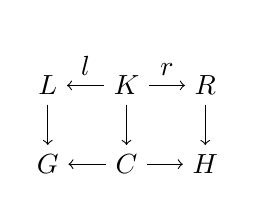
\begin{tikzpicture}[node distance=11mm]
          \node (I) at (0,0) {$K$};
          \node (L) at (-1,0) {$L$};
          \node (R) at (1,0) {$R$};
          \node (G) at (-1,-1) {$G$};
          \node (C) at (0,-1) {$C$};
          \node (H) at (1,-1) {$H$};
          \draw [->] (I) to node [label, above] {$l$} (L);
          \draw [->] (I) to node [label,above] {$r$} (R);
        %   \draw [->] (L) to node [label, right] {$m$} (G);
        \draw [->] (L) to node [label, right] {} (G);
          \draw [->] (I) to (C);
          \draw [->] (R) to (H);
          \draw [->] (C) to (G);
          \draw [->] (C) to (H);
        \end{tikzpicture}
        }
      \end{center}
\end{definition}
\begin{example}
    \label{wf:example:context_closure}
    Let the set of edge labels be $\Sigma \mathop{=} \{a,b\}$.
    Consider the following DPO rule:
    % in Example~\ref{ex:nwf:grsaa_rule}.
    % \begin{figure}[H]
    %  \centering 
    \begin{center}
      \resizebox{0.7\textwidth}{!}{
      \begin{tikzpicture}
          \graphbox{$L$}{0mm}{0mm}{34mm}{15mm}{2mm}{-5mm}{
              \coordinate (o) at (0mm,-3mm); 
              \node[draw,circle] (l1) at ($(o)+(-10mm,0mm)$) {1};
              \node[draw,circle] (l2) at ($(l1)+(2,0)$) {2};
              \node[draw,circle] (l3) at ($(l1)+(1,0)$) {3};
              \draw[->] (l1) -- (l3) node[midway,above] {$a$};
              \draw[->] (l3) -- (l2) node[midway,above] {$a$};
          }     
          \graphbox{$K$}{40mm}{0mm}{24mm}{15mm}{2mm}{-5mm}{
              \coordinate (o) at (5mm,-3mm); 
              \node[draw,circle] (l1) at ($(o)+(-10mm,0mm)$) {1};
              \node[draw,circle] (l2) at ($(l1)+(1,0)$) {2};
              % \node[draw,circle] (l3) at ($(l1)+(1,0)$) {$\ $};
              % \draw[->] (l1) -- (l3) node[midway,above] {$a$};
              % \draw[->] (l3) -- (l2) node[midway,above] {$a$};
          }    
          \graphbox{$R$}{70mm}{0mm}{45mm}{15mm}{2mm}{-5mm}{
              \coordinate (o) at (-5mm,-3mm); 
              \node[draw,circle] (l1) at ($(o)+(-10mm,0mm)$) {1};
              \node[draw,circle] (l2) at ($(l1)+(3,0)$) {2};
              \node[draw,circle] (l3) at ($(l1)+(1,0)$) {4};
              \node[draw,circle] (l4) at ($(l1)+(2,0)$) {5};
              \draw[->] (l1) -- (l3) node[midway,above] {$a$};
              \draw[->] (l3) -- (l4) node[midway,above] {$b$};
              \draw[->] (l4) -- (l2) node[midway,above] {$a$};
          }    
          \node () at (37mm,-8mm) {$\overset{l}{\leftarrowtail}$};
          \node () at (67mm,-8mm) {$\overset{r}{\rightarrowtail}$};
          % \draw[>->] (51mm,2mm) -- (52mm,3mm);
      \end{tikzpicture}
      }
    \end{center}
%       \caption{}
%       \label{fig:nwf:grsaa_rule}
%   \end{figure}
  \noindent and the following weighted type graph:
%    in Figure~\ref{fig:nwf:weighted_type_graph_grsaa} shown below
%   \begin{figure}[H]
%         \centering
\begin{center}
        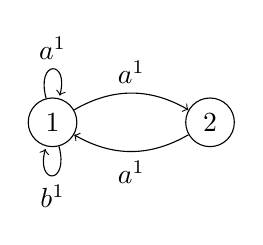
\begin{tikzpicture}
            \graphbox{}{0mm}{0mm}{32mm}{28mm}{-10mm}{-14mm}{
                \node[draw,circle] (1) at (0,0) {1};
                \node[draw,circle] (2) at (2,0) {2};
                \draw[->] (1) edge[loop above] node[midway, above] {$a^{1}$} (1) ;
                \draw[->] (1) edge[loop below] node[midway, below] {$b^{1}$} (1) ;
                \draw[->] (1) edge[bend left] node[midway, above] {$a^{1}$}  (2)  ;
                \draw[->] (2) edge[bend left] node[midway, below] {$a^{1}$} (1)   ;
            }
        \end{tikzpicture}
    %     \caption{}
    %     \label{fig:nwf:weighted_type_graph_grsaa}
    % \end{figure}
\end{center}
   Let $c$ be the morphism shown below.
%    in Figure~\ref{fig:nwf:context_closure_grsaa}. 
   Since for every match $m : L \mathop{\to} G$, there is a morphism $\alpha : G \mathop{\to} T$ such that $m \mathop{\star} \alpha \mathop{=} c$, the morphism $c$ is a context closure for the DPO rule in the type graph.
%   \begin{figure}[H]
%     \centering
    \begin{center}
    
    \resizebox{0.6\textwidth}{!}{
    \begin{tikzpicture}
      \graphbox{\( L \)}{-50mm}{0mm}{40mm}{40mm}{2mm}{-8mm}{
        \coordinate (o) at (0mm,-10mm); 
        \node[draw,circle] (l1) at ($(o)+(-10mm,0mm)$) {1};
        \node[draw,circle] (l2) at ($(l1)+(2,0)$) {2};
        \node[draw,circle] (l3) at ($(l1)+(1,0)$) {3};
        \draw[] (l1) -- (l3) node[midway,above] {$a$}; 
        \draw[] (l3) -- (l2) node[midway,above] {$a$};
    } 
        \graphbox{$T$}{0mm}{0mm}{40mm}{40mm}{-10mm}{-17mm}{
            % \node[draw,circle] (1) at (0,0) {$1\ 2\ 3$};
            % \node[draw,circle] (2) at (2,0) {};
            \coordinate (o) at (2mm,-3mm); 
            \node[draw,circle] (1) at ($(o)+(0,0mm)$) {$1\ 2\ 3$};
            \node[draw,circle] (2) at ($(o)+(2,0)$) {};
            \draw[->] (1) edge[loop above] node[midway, above] {$a^{1}$} (1) ;
            \draw[->] (1) edge[loop below] node[midway, below] {$b^{1}$} (1) ;
            \draw[->] (1) edge[bend left] node[midway, above] {$a^{1}$}  (2)  ;
            \draw[->] (2) edge[bend left] node[midway, below] {$a^{1}$} (1)   ;
        }
        \node () at (-5mm,-15mm) {$\overset{c}{\to}$};
    \end{tikzpicture}
    }
\end{center}  
\end{example} 

\subsection{Decreasing rules}
\label{sec:decreasing_rules}
%  This difference must exceed a fixed positive constant $\delta \mathop{\in} \mathbb{R}_{>0}$.
The following definition of decreasing rules from~\cite{endrullis2024generalized_arxiv_v2} classifies DPO rewriting rules.

\begin{definition}[\cite{endrullis2024generalized_arxiv_v2}]
    \label{wf:def:decreasing_rule}
    Let $\mathcal{T} \mathop{=} (T,\mathbb{E}, (S, \mathop{\oplus}, \mathop{\odot}, 0_S, 1_S, \prec, \mathop{\preceq}),w)$ be a finitary weighted type graph, \(\mathfrak{F}\) a DPO rewriting framework, $\rho \mathop{=} (L \overset{l}{\leftarrow} K \overset{r}{\rightarrow} R)$ a DPO rewriting rule.

    \noindent
    The rule $\rho$ is said to be \textbf{weakly decreasing} with respect to $\mathcal{T}$ in $\mathfrak{F}$ if 
            for every $t_K : K \mathop{\to} T$, the following inequality holds:
                $$ 
                  w_\mathcal{T}(\{l \mathop{\star} - \mathop{=} t_K\}) \mathop{\succeq} w_\mathcal{T}(\{r\star - \mathop{=} t_K\}).$$
           
    \noindent
    The rule $\rho$ is said to be \textbf{uniformly decreasing} with respect to $\mathcal{T}$ in $\mathfrak{F}$ if the following conditions holds:
        \begin{itemize}
            \item[]- there is a context closure $c_\rho$ for $\rho$ and $\mathcal{T}$ in $\mathfrak{F}$, 
            \item[]- for every $t_K : K \mathop{\to} T$,
            \begin{itemize}
                \item[] $\bullet$ $\{l \mathop{\star} - \mathop{=} t_K\} \mathop{=} \emptyset \mathop{=} \{r \mathop{\star} - \mathop{=} t_K\}$, or
                \item[] $\bullet$ $w_\mathcal{T}(\{l \mathop{\star} - \mathop{=} t_K\}) 
                        \mathop{\succ}   w_\mathcal{T}(\{r \mathop{\star} - \mathop{=} t_K\}) $.
            \end{itemize}
        \end{itemize}  
         
    \noindent
   If $S$ is moreover strictly monotonic, we say the rule $\rho$ is
            \textbf{closure decreasing} with respect to $\mathcal{T}$ in $\mathfrak{F}$ if the following holds:
            \begin{itemize}
                \item[]- $\rho$ is weakly decreasing,
                \item[]- there is a context closure $c_\rho$ for $\rho$ and $\mathcal{T}$ in $\mathfrak{F}$,
                \item[]- $w_\mathcal{T}(\{l \mathop{\star} - \mathop{=} t_K\})  
                \mathop{\succ}  w_\mathcal{T}(\{r \mathop{\star} - \mathop{=} t_K\})$ for $t_K \mathop{=} l \mathop{\star} c_\rho$.
            \end{itemize}
\end{definition}

\begin{example}
    \label{wf:example:decreasing_rule}
    Consider the following DPO rule:
    % in Example~\ref{ex:nwf:grsaa_rule_2}
    % \begin{figure}[H]
    %   \centering
    \begin{center}
      \resizebox{0.7\textwidth}{!}{
      \begin{tikzpicture}
          \graphbox{$L$}{0mm}{0mm}{34mm}{15mm}{2mm}{-5mm}{
              \coordinate (o) at (0mm,-3mm); 
              \node[draw,circle] (l1) at ($(o)+(-10mm,0mm)$) {1};
              \node[draw,circle] (l2) at ($(l1)+(2,0)$) {2};
              \node[draw,circle] (l3) at ($(l1)+(1,0)$) {3};
              \draw[->] (l1) -- (l3) node[midway,above] {$a$};
              \draw[->] (l3) -- (l2) node[midway,above] {$a$};
          }     
          \graphbox{$K$}{40mm}{0mm}{24mm}{15mm}{2mm}{-5mm}{
              \coordinate (o) at (5mm,-3mm); 
              \node[draw,circle] (l1) at ($(o)+(-10mm,0mm)$) {1};
              \node[draw,circle] (l2) at ($(l1)+(1,0)$) {2};
              % \node[draw,circle] (l3) at ($(l1)+(1,0)$) {$\ $};
              % \draw[->] (l1) -- (l3) node[midway,above] {$a$};
              % \draw[->] (l3) -- (l2) node[midway,above] {$a$};
          }    
          \graphbox{$R$}{70mm}{0mm}{45mm}{15mm}{2mm}{-5mm}{
              \coordinate (o) at (-5mm,-3mm); 
              \node[draw,circle] (l1) at ($(o)+(-10mm,0mm)$) {1};
              \node[draw,circle] (l2) at ($(l1)+(3,0)$) {2};
              \node[draw,circle] (l3) at ($(l1)+(1,0)$) {4};
              \node[draw,circle] (l4) at ($(l1)+(2,0)$) {5};
              \draw[->] (l1) -- (l3) node[midway,above] {$a$};
              \draw[->] (l3) -- (l4) node[midway,above] {$b$};
              \draw[->] (l4) -- (l2) node[midway,above] {$a$};
          }    
          \node () at (37mm,-8mm) {$\overset{l}{\leftarrowtail}$};
          \node () at (67mm,-8mm) {$\overset{r}{\rightarrowtail}$};
          % \draw[>->] (51mm,2mm) -- (52mm,3mm);
      \end{tikzpicture}
      }
%       \caption{}
%       \label{ex:nwf:grsaa_rule_2}
%   \end{figure} 
    \end{center}
  \noindent and the following weighted type graph
%    in Figure~\ref{fig:nwf:weighted_type_graph_grsaa_2} 
   over the natural arithmetic semiring $\mathfrak{N} \mathop{=} (\mathbb{N},+,*,0,1,<,\leq)$.
%   \begin{figure}[H]
%     \centering
\begin{center}
        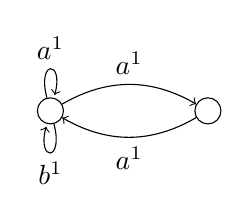
\begin{tikzpicture}
            \graphbox{}{0mm}{0mm}{32mm}{26mm}{-10mm}{-14mm}{
                \node[draw,circle] (1) at (0,0) {};
                \node[draw,circle] (2) at (2,0) {};
                \draw[->] (1) edge[loop above] node[midway, above] {$a^{1}$} (1) ;
                \draw[->] (1) edge[loop below] node[midway, below] {$b^{1}$} (1) ;
                \draw[->] (1) edge[bend left] node[midway, above] {$a^{1}$}  (2)  ;
                \draw[->] (2) edge[bend left] node[midway, below] {$a^{1}$} (1)   ;
            }
        \end{tikzpicture}
    %     \caption{}
    %     \label{fig:nwf:weighted_type_graph_grsaa_2}
    % \end{figure}
    \end{center}
     There are 4 morphisms $t_K^{11}, t_K^{12}, t_K^{21}, t_K^{22}$ from $K$ to $T$:
    %   in Figure~\ref{fig:nwf:grsaa_rule_morphisms}.

    % \begin{figure}[H]
    %     \centering
    \begin{center}
        \resizebox{0.6\textwidth}{!}{
            \begin{tikzpicture}
            \graphbox{\( K \)}{-50mm}{0mm}{40mm}{30mm}{2mm}{-6mm}{
                \coordinate (o) at (0mm,-10mm); 
                \node[draw,circle] (l1) at ($(o)+(-10mm,0mm)$) {1};
                \node[draw,circle] (l2) at ($(l1)+(2,0)$) {2};
                % \node[draw,circle] (l3) at ($(l1)+(1,0)$) {3};
                % \draw[] (l1) -- (l3) node[midway,above] {$a$};
                % \draw[] (l3) -- (l2) node[midway,above] {$a$};
            } 
                \graphbox{$T$}{0mm}{0mm}{40mm}{30mm}{-10mm}{-15mm}{
                    \node[draw,circle] (1) at (0,0) {$1\ 2$};
                    \node[draw,circle] (2) at (2,0) {};
                    \draw[->] (1) edge[loop above] node[midway, above] {$a$} (1) ;
                    \draw[->] (1) edge[loop below] node[midway, below] {$b$} (1) ;
                    \draw[->] (1) edge[bend left] node[midway, above] {$a$}  (2)  ;
                    \draw[->] (2) edge[bend left] node[midway, below] {$a$} (1)   ;
                }
                \node () at (-5mm,-15mm) {$\overset{t_K^{11}}{\to}$};
            \end{tikzpicture}
            } 

            \resizebox{0.6\textwidth}{!}{
            \begin{tikzpicture}
                \graphbox{\( K \)}{-50mm}{0mm}{40mm}{28mm}{2mm}{-6mm}{
                \coordinate (o) at (0mm,-10mm); 
                \node[draw,circle] (l1) at ($(o)+(-10mm,0mm)$) {1};
                \node[draw,circle] (l2) at ($(l1)+(2,0)$) {2};
                % \node[draw,circle] (l3) at ($(l1)+(1,0)$) {3};
                % \draw[] (l1) -- (l3) node[midway,above] {$a$};
                % \draw[] (l3) -- (l2) node[midway,above] {$a$};
            } 
                \graphbox{$T$}{0mm}{0mm}{40mm}{28mm}{-10mm}{-15mm}{
                    \node[draw,circle] (1) at (0,0) {$1$};
                    \node[draw,circle] (2) at (2,0) {2};
                    \draw[->] (1) edge[loop above] node[midway, above] {$a$} (1) ;
                    \draw[->] (1) edge[loop below] node[midway, below] {$b$} (1) ;
                    \draw[->] (1) edge[bend left] node[midway, above] {$a$}  (2)  ;
                    \draw[->] (2) edge[bend left] node[midway, below] {$a$} (1)   ;
                }
                \node () at (-5mm,-15mm) {$\overset{t_K^{12}}{\to}$};
            \end{tikzpicture}
            }
            
            \resizebox{0.6\textwidth}{!}{
            \begin{tikzpicture}
                \graphbox{\( K \)}{-50mm}{0mm}{40mm}{28mm}{2mm}{-6mm}{
                \coordinate (o) at (0mm,-10mm); 
                \node[draw,circle] (l1) at ($(o)+(-10mm,0mm)$) {1};
                \node[draw,circle] (l2) at ($(l1)+(2,0)$) {2};
                % \node[draw,circle] (l3) at ($(l1)+(1,0)$) {3};
                % \draw[] (l1) -- (l3) node[midway,above] {$a$};
                % \draw[] (l3) -- (l2) node[midway,above] {$a$};
            } 
                \graphbox{$T$}{0mm}{0mm}{40mm}{28mm}{-10mm}{-15mm}{
                    \node[draw,circle] (1) at (0,0) {2};
                    \node[draw,circle] (2) at (2,0) {1};
                    \draw[->] (1) edge[loop above] node[midway, above] {$a$} (1) ;
                    \draw[->] (1) edge[loop below] node[midway, below] {$b$} (1) ;
                    \draw[->] (1) edge[bend left] node[midway, above] {$a$}  (2)  ;
                    \draw[->] (2) edge[bend left] node[midway, below] {$a$} (1)   ;
                }
                \node () at (-5mm,-15mm) {$\overset{t_K^{21}}{\to}$};
            \end{tikzpicture}
            }

            \resizebox{0.6\textwidth}{!}{
            \begin{tikzpicture}
                \graphbox{\( K \)}{-50mm}{0mm}{40mm}{28mm}{2mm}{-6mm}{
                \coordinate (o) at (0mm,-10mm); 
                \node[draw,circle] (l1) at ($(o)+(-10mm,0mm)$) {1};
                \node[draw,circle] (l2) at ($(l1)+(2,0)$) {2};
                % \node[draw,circle] (l3) at ($(l1)+(1,0)$) {3};
                % \draw[] (l1) -- (l3) node[midway,above] {$a$};
                % \draw[] (l3) -- (l2) node[midway,above] {$a$};
            } 
                \graphbox{$T$}{0mm}{0mm}{40mm}{26mm}{-10mm}{-15mm}{
                    \node[draw,circle] (1) at (0,0) {};
                    \node[draw,circle] (2) at (2,0) {$1\ 2$};
                    \draw[->] (1) edge[loop above] node[midway, above] {$a$} (1) ;
                    \draw[->] (1) edge[loop below] node[midway, below] {$b$} (1) ;
                    \draw[->] (1) edge[bend left] node[midway, above] {$a$}  (2)  ;
                    \draw[->] (2) edge[bend left] node[midway, below] {$a$} (1)   ;
                }
                \node () at (-5mm,-15mm) {$\overset{t_K^{22}}{\to}$};
            \end{tikzpicture}
            }
    %     \caption{}
    %     \label{fig:nwf:grsaa_rule_morphisms}
    %   \end{figure}
    \end{center}
    The set $\{l \mathop{\star} - \mathop{=} t_K^{11}\}$ consists of two morphisms $h_{11}^1$ and $h_{11}^2$:
    % shown in Figure~\ref{fig:nwf:grsaa_rule_morphisms_22}.
    % \begin{figure}[H]
    %     \centering
    \begin{center}
        \resizebox{0.6\textwidth}{!}{
        \begin{tikzpicture}
          \graphbox{\( L \)}{-50mm}{0mm}{40mm}{35mm}{2mm}{-6mm}{
            \coordinate (o) at (0mm,-10mm); 
            \node[draw,circle] (l1) at ($(o)+(-10mm,0mm)$) {1};
            \node[draw,circle] (l2) at ($(l1)+(2,0)$) {2};
            \node[draw,circle] (l3) at ($(l1)+(1,0)$) {3};
            \draw[] (l1) -- (l3) node[midway,above] {$a$};
            \draw[] (l3) -- (l2) node[midway,above] {$a$};
        } 
            \graphbox{$T$}{0mm}{0mm}{40mm}{35mm}{-8mm}{-17mm}{
                \node[draw,circle] (1) at (0,0) {$1\ 2$};
                \node[draw,circle] (2) at (2,0) {3};
                \draw[->] (1) edge[loop above] node[midway, above] {$a^{1}$} (1) ;
                \draw[->] (1) edge[loop below] node[midway, below] {$b^{1}$} (1) ;
                \draw[->] (1) edge[bend left] node[midway, above] {$a^{1}$}  (2)  ;
                \draw[->] (2) edge[bend left] node[midway, below] {$a^{1}$} (1)   ;
            }
            \node () at (-5mm,-15mm) {$\overset{h_{11}^1}{\to}$};
        \end{tikzpicture}
        }

        \resizebox{0.6\textwidth}{!}{
            \begin{tikzpicture}
              \graphbox{\(L\)}{-50mm}{0mm}{40mm}{37mm}{2mm}{-10mm}{
                \coordinate (o) at (0mm,-10mm); 
                \node[draw,circle] (l1) at ($(o)+(-10mm,0mm)$) {1};
                \node[draw,circle] (l2) at ($(l1)+(2,0)$) {2};
                \node[draw,circle] (l3) at ($(l1)+(1,0)$) {3};
                \draw[] (l1) -- (l3) node[midway,above] {$a$};
                \draw[] (l3) -- (l2) node[midway,above] {$a$};
            } 
                \graphbox{$T$}{0mm}{0mm}{40mm}{37mm}{-8mm}{-20mm}{
                    \node[draw,circle] (1) at (0,0) {$1\ 2\ 3$};
                    \node[draw,circle] (2) at (2,0) {};
                    \draw[->] (1) edge[loop above] node[midway, above] {$a^{1}$} (1) ;
                    \draw[->] (1) edge[loop below] node[midway, below] {$b^{1}$} (1) ;
                    \draw[->] (1) edge[bend left] node[midway, above] {$a^{1}$}  (2)  ;
                    \draw[->] (2) edge[bend left] node[midway, below] {$a^{1}$} (1)   ;(1)   ;
                }
                \node () at (-5mm,-15mm) {$\overset{h_{11}^2}{\to}$};
            \end{tikzpicture}
            }
    \end{center}
    %     \caption{}
    %     \label{fig:nwf:grsaa_rule_morphisms_22}
    %   \end{figure}
    Therefore, we have \begin{flalign*}
        w_\mathcal{T}(\{l \mathop{\star} - \mathop{=} t_K^{11}\})
        =&w_\mathcal{T}(\{h_{11}^1, h_{11}^2\})\\
        =&w_\mathcal{T}(h_{11}^1)\mathop{+}w_\mathcal{T}(h_{11}^2) \\
        =&(1^1 * 1^1)+(1^1 * 1^1)\\
        =&2.
    \end{flalign*}
    The set $\{r \mathop{\star} - \mathop{=} t_K^{11}\}$ has one morphism $h_{11}^3$:
    % in Example~\ref{wf:example:context_closure_grs_aa}.
    % \begin{figure}[H]
    %     \centering
    \begin{center}
        \resizebox{0.7\textwidth}{!}{
        \begin{tikzpicture}
          \graphbox{\( R \)}{-55mm}{0mm}{45mm}{44mm}{1mm}{-22mm}{
            \coordinate (o) at (-5mm,-3mm); 
            \node[draw,circle] (l1) at ($(o)+(-10mm,0mm)$) {1};
            \node[draw,circle] (l2) at ($(l1)+(3,0)$) {2};
            \node[draw,circle] (l3) at ($(l1)+(1,0)$) {4};
            \node[draw,circle] (l4) at ($(l1)+(2,0)$) {5};
            \draw[->] (l1) -- (l3) node[midway,above] {$a$};
            \draw[->] (l3) -- (l4) node[midway,above] {$b$};
            \draw[->] (l4) -- (l2) node[midway,above] {$a$};
        } 
            \graphbox{$T$}{0mm}{0mm}{40mm}{44mm}{-10mm}{-22mm}{
                \node[draw,circle] (1) at (0,0) {$1\ 2\ 4\ 5$};
                \node[draw,circle] (2) at (2,0) {};
                \draw[->] (1) edge[loop above] node[midway, above] {$a^{1}$} (1) ;
                \draw[->] (1) edge[loop below] node[midway, below] {$b^{1}$} (1) ;
                \draw[->] (1) edge[bend left] node[midway, above] {$a^{1}$}  (2)  ;
                \draw[->] (2) edge[bend left] node[midway, below] {$a^{1}$} (1)   ;
            }
            \node () at (-5mm,-19mm) {$\overset{h_{11}^3}{\to}$};
        \end{tikzpicture}
        }
    \end{center}
        %     \caption{}
    %     \label{fig:example:context_closure_grs_aa}
    %   \end{figure}
    Therefore, we have: 
        $$w_\mathcal{T}(\{r \mathop{\star} - \mathop{=} t_K^{11}\}) \mathop{=} w_\mathcal{T}(h_{11}^3) \mathop{=} 1^1 * 1^1 * 1 ^ 1 \mathop{=} 1.$$ 
    The following inequality follows
     $$w_\mathcal{T}(\{l \mathop{\star} - \mathop{=} t_K^{11}\}) \mathop{=} 2 \mathop{\geq} 1 \mathop{=} w_\mathcal{T}(\{r \mathop{\star} - \mathop{=} t_K^{11}\}).$$

    Similarly, we can check that
        \begin{itemize}
            \item $w_\mathcal{T}(\{l \mathop{\star} - \mathop{=} t_K^{12}\}) \mathop{=} 1 \mathop{\geq} 1 \mathop{=} w_\mathcal{T}(\{r \mathop{\star} - \mathop{=} t_K^{12}\})$, and
            \item $w_\mathcal{T}(\{l \mathop{\star} - \mathop{=} t_K^{21}\}) \mathop{=} 1 \mathop{\geq} 1 \mathop{=} w_\mathcal{T}(\{r \mathop{\star} - \mathop{=} t_K^{21}\})$, and
            \item $w_\mathcal{T}(\{l \mathop{\star} - \mathop{=} t_K^{22}\}) \mathop{=} 1 \mathop{\geq} 1 \mathop{=} w_\mathcal{T}(\{r \mathop{\star} - \mathop{=} t_K^{22}\})$.
        \end{itemize}  
     The rule is therefore weakly decreasing.

    The morphism $c$ illustrated below is a context closure for the DPO rule and the weighted type graph shown above, as explained in Example~\ref{wf:example:decreasing_rule}.
    % \begin{figure}[H]
    % \centering    
    \begin{center}
    \resizebox{0.6\textwidth}{!}{
    \begin{tikzpicture}
      \graphbox{\( L \)}{-50mm}{0mm}{40mm}{40mm}{2mm}{-8mm}{
        \coordinate (o) at (0mm,-10mm); 
        \node[draw,circle] (l1) at ($(o)+(-10mm,0mm)$) {1};
        \node[draw,circle] (l2) at ($(l1)+(2,0)$) {2};
        \node[draw,circle] (l3) at ($(l1)+(1,0)$) {3};
        \draw[] (l1) -- (l3) node[midway,above] {$a$}; 
        \draw[] (l3) -- (l2) node[midway,above] {$a$};
    } 
        \graphbox{$T$}{0mm}{0mm}{40mm}{40mm}{-10mm}{-17mm}{
            % \node[draw,circle] (1) at (0,0) {$1\ 2\ 3$};
            % \node[draw,circle] (2) at (2,0) {};
            \coordinate (o) at (2mm,-3mm); 
            \node[draw,circle] (1) at ($(o)+(0,0mm)$) {$1\ 2\ 3$};
            \node[draw,circle] (2) at ($(o)+(2,0)$) {};
            \draw[->] (1) edge[loop above] node[midway, above] {$a^{1}$} (1) ;
            \draw[->] (1) edge[loop below] node[midway, below] {$b^{1}$} (1) ;
            \draw[->] (1) edge[bend left] node[midway, above] {$a^{1}$}  (2)  ;
            \draw[->] (2) edge[bend left] node[midway, below] {$a^{1}$} (1)   ;
        }
        \node () at (-5mm,-15mm) {$\overset{c}{\to}$};
    \end{tikzpicture}
    }
\end{center}
    Since the following conditions hold:
        \begin{itemize}
            \item $t_K^{11} \mathop{=} l \mathop{\star} c$, and
            \item $w_\mathcal{T}(\{l \mathop{\star} - \mathop{=} t_K^{11}\}) \mathop{=} 2 \mathop{>} 1 \mathop{=} w_\mathcal{T}(\{r \mathop{\star} - \mathop{=} t_K^{11}\})$.
        \end{itemize}
       we conclude that the rule is closure decreasing since the semiring is strictly monotonic.
\end{example} 
 
\subsection{Termination Criterion}
\label{wf:sec:termination}
Finally, we can state the main result from~\cite{endrullis2024generalized_icgt}.
\begin{theorem}[Termination of DPO rewriting system] 
    \label{wf:thm:termination_grs}
    Let $\mathcal{A}$ and $\mathcal{B}$ be sets of DPO rewriting rules, $\mathcal{T} \mathop{=} (T,\mathbb{E}, (S, \mathop{\oplus}, \mathop{\odot}, 0_S, 1_S, \prec, \leq), w)$ a finitary weighted type graph and $\mathfrak{F}$ a DPO rewriting framework such that

        \begin{itemize} 
            \item \(\operatorname{left}(\Delta)\) is weighable with \(\mathcal{T}\),
            \item \(\operatorname{right}(\Delta)\) is bounded above by \(\mathcal{T}\). 
        \end{itemize}
    for every rule $\rho \mathop{\in} (\mathcal{A }\mathop{\cup} \mathcal{B })$ and every double pushout diagram  
        $\Delta \mathop{\in} \mathfrak{F}(\rho)$. If the following conditions hold:
    \begin{enumerate}
        \item either every $\rho \mathop{\in} \mathcal{A}$ is uniformly decreasing or every $\rho \mathop{\in} \mathcal{A}$ is closure decreasing, and
        \item every rule $\rho \mathop{\in} \mathcal{B}$ is weakly decreasing,
    \end{enumerate}
    then $\mathop{\Rightarrow}_{\mathcal{A},\mathfrak{F}}$ is \textbf{terminating} relative to $\mathop{\Rightarrow}_{\mathcal{B},\mathfrak{F}}$.
\end{theorem} 
\begin{example} 
    \label{wf:example:termination}
    Termination of the DPO rule in Example~\ref{ex:grsaa} can be established using Theorem~\ref{wf:thm:termination_grs} together with the weighted type graph in Example~\ref{wf:example:weighted_type_graph} over the natural arithmetic semiring $\mathfrak{N} \mathop{=} (\mathbb{N},+,*,0_\mathbb{R},1_\mathbb{N},<,\leq)$. It is closure decreasing as explained in Example~\ref{wf:example:decreasing_rule}.
\end{example}
